%-----------------------------------------------
% Template para criação de resumos de projectos/dissertação
% jlopes AT fe.up.pt,   Fri Jul  3 11:08:59 2009
%-----------------------------------------------

\documentclass[9pt,a4paper]{extarticle}

%% English version: comment first, uncomment second
\usepackage[portuguese]{babel}  % Portuguese
%\usepackage[english]{babel}     % English
\usepackage{graphicx}           % images .png or .pdf w/ pdflatex OR .eps w/ latex
\usepackage{times}              % use Times type-1 fonts
\usepackage[utf8]{inputenc}     % 8 bits using UTF-8
\usepackage{url}                % URLs
\usepackage{multicol}           % twocolumn, etc
\usepackage{float}              % improve figures & tables floating
\usepackage[tableposition=top]{caption} % captions
\usepackage{mathtools}
%% English version: comment first (maybe)
\usepackage{indentfirst}        % portuguese standard for paragraphs
%\usepackage{parskip}

%% page layout
\usepackage[a4paper,margin=30mm,noheadfoot]{geometry}

%% space between columns
\columnsep 12mm

%% headers & footers
\pagestyle{empty}

%% figure & table caption
\captionsetup{figurename=Fig.,tablename=Tab.,labelsep=endash,font=bf,skip=.5\baselineskip}

%% heading
\makeatletter
\renewcommand*{\@seccntformat}[1]{%
  \csname the#1\endcsname.\quad
}
\makeatother

%% avoid widows and orphans
\clubpenalty=300
\widowpenalty=300


\begin{document}

\title{\vspace*{-8mm}\textbf{\textsc{Software Repository Mining Analytics to Estimate Software Component Reliability}}}
\author{\emph{André Freitas - freitas.andre@fe.up.pt}\\[2mm]
\small{Dissertação realizada sob a orientação do \emph{Prof.\ Rui Maranhão e Alexandre Perez}}}
\date{}
\maketitle
%no page number
\thispagestyle{empty}

\vspace*{-4mm}\noindent\rule{\textwidth}{0.4pt}\vspace*{4mm}

\begin{multicols}{2}

\section{Motivação}\label{sec:motiva}
O Software desempenha um papel fundamental na nossa sociedade e na nossa rotina
diária, pois dependemos de aplicações para comunicar, gerir informação, etc.
O desenvolvimento de Software é relativamente complexo e o custo de
corrigir bugs representa até 90\% do custo do projeto \cite{Servant1}.

Os repositórios de Software têm informação valiosa que pode ser explorada com
técnicas de \emph{Machine Learning} e de \emph{Analytics} para suportar modelos
de previsão de defeitos de \emph{Software}.

O \emph{Crowbar} \footnote{\url{http://crowbar.io/}} é uma ferramenta de localização
automática de falhas, que após a execução de uma bateria de testes, estima os
componentes faltosos. O algoritmo \emph{Barinel} usado nesta ferramenta usa estimativas
estáticas \cite{Abreu:2009:SMF:1747491.1747511}. Estas podem ser substituídas
por estimativas dinâmicas provenientes do resultado da previsão de defeitos, de
maneira a melhorar a qualidade do diagnóstico das falhas.


\section{Objectivos}\label{sec:goals}

Os principais objetivos são:

\begin{itemize}
\item Prever defeitos a partir de repositórios de \emph{Software} ao aprender quais
são as variáveis mais importantes a analisar e criar um modelo de previsão
baseado nas técnicas existentes;
\item Melhorar o diagnóstico de falhas no \emph{Crowbar} com base nos resultados
da previsão de defeitos.
\end{itemize}

\section{Descrição do Trabalho}\label{sec:work}
Foi implementada uma ferramenta em \emph{Python} denominada \emph{Schwa}, que é capaz de
analisar repositórios \emph{Git} e estimar a probabilidade de um determinado componente
possuir defeitos. Por exemplo, o \emph{Schwa} consegue estimar que um determinado
ficheiro tem uma certa de probabilidade de ter um defeito. Caso o ficheiro for
de código \emph{Java}, a granularidade é até ao método, ou seja, é possível estimar
a probabilidade de classes e métodos serem defeituosos.

\subsection{Instalação}
O \emph{Schwa} está disponível livremente no \emph{Github}
\footnote{\url{https://github.com/andrefreitas/schwa}} e pode ser facilmente
instalado por:
\begin{verbatim}
    pip install schwa --pre
\end{verbatim}

\subsection{Utilização da ferramenta}
O \emph{Schwa} pode ser invocado como um utilitário de linha de comandos com a
seguinte sintaxe:

\begin{verbatim}
  schwa git/repo/path [--commits COMMITS]
\end{verbatim}

O número de \emph{commits} é opcional para o caso de se pretender analisar
apenas as últimas alterações. É apresentado o relatório na fig. \ref{fig:sunburst}.

\begin{figure}[H]
\centerline{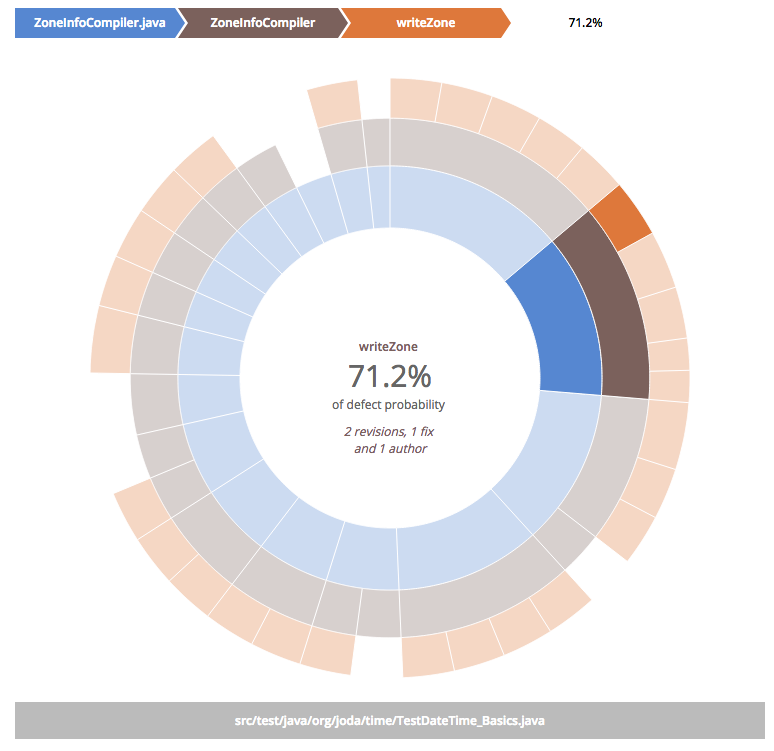
\includegraphics[scale=.25]{sunburst.png}}
\caption{Relatório do Schwa}
\label{fig:sunburst}
\end{figure}

No gráfico da fig. \ref{fig:sunburst} é possível inspecionar os componentes
(ficheiros, classes ou métodos) de um modo hierárquico. Aparece no centro a
estimativa da probabilidade de defeito juntamente com o os valores das métricas
recolhidas, que são o número de revisões, correções e de autores do componente.

\subsection{Extração}
A primeira fase do processo do \emph{Schwa} é a extração de dados do repositório que
sejam relevantes para a análise. Com recurso à biblioteca \emph{GitPython},
\footnote{\url{https://github.com/gitpython-developers/GitPython}}
em cada \emph{commit} extraimos a mensagem, o autor, o \emph{timestamp} e a lista dos
componentes alterados.

De maneira a interpretar as alterações de código \emph{Java}, foi usada a biblioteca
\emph{Plyj}\footnote{\url{https://github.com/musiKk/plyj}}, que foi modificada
para incluir a informação do número das linhas nas classes e métodos.

\subsection{Análise}
A análise é feita tendo em conta os seguintes princípios:

\begin{itemize}
\item \textbf{Princípio das revisões} Quantas mais revisões tem um componente,
maior é a sua probabilidade de defeito\cite{859533};

\item \textbf{Princípio das correções} Existe uma correlação entre defeitos do
passado e defeitos no futuro \cite{Zimmermann:2007:PDE:1268984.1269057};

\item \textbf{Princípio dos autores} O número de autores é uma variável
preditiva de defeitos \cite{Moser:2008:CAE:1368088.1368114,D'Ambros:2012:EDP:2318097.2318149}.
\end{itemize}


As variáveis utilizadas na análise são revisões, correções e autores e são
recolhidas através do seguinte algoritmo:

\begin{verbatim}
For each commit in the repository
  twr = compute twr
  For each component in the commit
    component.revisions += twr
    IF commit is bug fix
        component.fixes += twr
    If is new author
        component.authors += twr
\end{verbatim}

Em vez de se usar contadores, é usada a função \emph{Time-Weighted-Risk} (TWR) que
tem um valor máximo quando a alteração do componente é recente. Esta função
recebe um \emph{timestamp} normalizado \cite{Chris2013}.

\begin{equation}
twr(t_i) = \frac{1}{1 + e^{-12t_i + 12 }}
\end{equation}

\subsection{Modelo de previsão de defeitos}
É calculado primeiro um \emph{score} para cada componente:
\begin{equation}
\begin{multlined}score = revisions * revisions_{weight} \\
+ fixes * fixes_{weight} \\
+ authors * authors_{weight} \\
\end{multlined}
\end{equation}

O \emph{score} é então normalizado:

\begin{equation}
defect_{probability} = 1 - e^{-score}
\end{equation}

\subsection{Experiências}
Desenvolvemos um modelo de aprendizagem dos pesos das variáveis (revisões,
correções e autores) com algoritmos genéticos. Após o \emph{Schwa} aprender com
projetos académicos, \emph{Open Source} e empresariais, concluímos que os pesos
variam de projeto para projeto.

Ao usarmos o \emph{Schwa} no \emph{Crowbar}, conseguimos reduzir o tempo de
diagnóstico. No projecto \emph{Joda Time} reduzimos de 1 hora para menos de 1 minuto.

\section{Conclusões}\label{sec:conclui}
Conseguimos criar uma técnica capaz de prever defeitos de componentes de
\emph{Software} com base na análise de repositórios \emph{Git} com um relatório visual.

As técnicas atuais de revisão de código podem beneficiar da utilização do \emph{Schwa},
pois permite aos programadores focarem os seus recursos onde os defeitos estão.

%%English version: comment first, uncomment second
\bibliographystyle{unsrt-pt}  % numeric, unsorted refs
%\bibliographystyle{unsrt}  % numeric, unsorted refs
\bibliography{refs}

\end{multicols}

\end{document}
